
% this file is called up by thesis.tex
% content in this file will be fed into the main document

%: ----------------------- introduction file header -----------------------
\begin{savequote}[50mm]
Historical methodology, as I see it, is a product of common sense applied to circumstances. 
\qauthor{Samuel E. Morison}
\end{savequote}


\chapter{Método para la evaluación de competencias genéricas}
\label{cha:Overall methodology}

% the code below specifies where the figures are stored
\ifpdf
    \graphicspath{{4_overall_methodology/figures/PNG/}{4_overall_methodology/figures/PDF/}{4_overall_methodology/figures/}}
\else
    \graphicspath{{4_overall_methodology/figures/EPS/}{4_overall_methodology/figures/}}
\fi


%------------------------------------------------------------------------- 

En este capítulo se propone un método para la evaluación de competencias genéricas de los estudiantes a partir de indicadores obtenidos del registro de interacciones de las actividades de aprendizaje. El capítulo comienza con una introducción para sentar las bases del método. En segundo lugar, se contextualiza y describe el método. En tercer lugar, se continúa con las características y los requisitos que debe cumplir el método. Y finalmente, se presenta su implementación en tres actividades de aprendizaje diferentes: wikis, VLEs y mundos virtuales.

\section{Introducción}

Se podría decir que hoy en día los entornos virtuales constituyen una pieza fundamental en cualquier contexto en el que se impartan cursos. Mientras que en los cursos virtuales, los VLEs son el único entorno de trabajo posible, en los cursos presenciales, tantos los VLEs como otras herramientas virtuales actúan como soporte virtual de las clases, proporcionando multitud de actividades de aprendizaje. 

En el VLE por ejemplo, los estudiantes pasan a diario por sus páginas. Por un lado, habrá estudiantes que entren en el VLE varias veces al día a consultar cualquier novedad y que sólo permanezcan 20 segundos en el mismo. Mientras que por otro lado, habrá estudiantes que entren una vez a la semana pero estén dos horas navegando por el VLE. Y entre un tipo de estudiante y otro, habrá tantas maneras de actuar de los estudiantes en el VLE como estudiantes haya. 

Todas las acciones de los estudiantes quedan almacenadas en el registro de las actividades de aprendizaje, y estos registros podrían ser analizados para comprender el proceso de aprendizaje que se está desarrollando. El \emph{learning analytics} es un área de investigación del aprendizaje mejorado por la tecnología (TEL, del inglés \emph{Technology Enhanced Learning}) que está enfocado en el desarrollo de métodos para analizar y detectar patrones en los datos recogidos en los entornos educativos y aprovecharlos para mejorar el aprendizaje~\cite{chatti2014learning}.

En esta tesis se propone que, a partir de este método, los profesores puedan detectar patrones de comportamiento de los estudiantes a partir de la actividad de éstos en las actividades de aprendizaje, y puedan basarse en dichos patrones para establecer indicadores del desempeño de los estudiantes en ciertas competencias genéricas. 

A continuación se detallará el método, se describirán sus requisitos y se mostrará su implementación en diferentes actividades de aprendizaje.

% ---- Comentarios ----------
% Hay que hablar en capítulos anteriores de registros en actividades de aprendizaje y no en el VLE
% Porque aquí las actividades de aprendizaje son 3: wiki, VLE y WV.


\section{Método: Ciclo de contraste de hipótesis}

\subsection{Contexto}

Los estudiantes comienzan a dejar constancia de su actividad en los entornos virtuales desde el momento en que acceden al entorno. El registro del sistema lo almacena todo, tanto la participación activa del estudiante, escribiendo y respondiendo mensajes en los foros o enviando actividades, como la participación pasiva, cuando simplemente se lee una página, se leen los mensajes del foro o se descargan los apuntes. 

Los programas de las asignaturas incluyen las competencias genéricas de las que los estudiantes deben ser evaluados. Los profesores pueden plantear actividades en los entornos virtuales con la intención no sólo de evaluar ciertas habilidades de los estudiantes, sino también de provocar comportamientos en los estudiantes y ver cómo afrontan ciertas situaciones. El fin de conocer el modo de proceder de los estudiantes es encontrar patrones de comportamiento que puedan ser interpretados como un indicador del desempeño de alguna competencia genérica.

Para evaluar una competencia genérica dada, el profesor podrá diseñar una evaluación a partir de la información relativa a los registros de los entornos de aprendizaje. Aquí comienza el  \emph{ciclo de contraste de hipótesis}. 

%Ese diseño será procesado por el sistema que implementa el método y que terminará devolviendo la información al profesor. El resultado de aplicar el diseño será un indicador que el profesor podrá utilizar para la evaluación de la competencia genérica.


%También se puede dar el caso de que el profesor considere que el indicador no es válido para la evaluación de la competencia genérica. También puede que aunque le sea válido pero considere que un rediseño del mismo le permitirá afinar más en cuánto al objetivo de evaluación de competencia genérica que se marcó. El profesor podría diseñar una nueva evaluación a partir de la información contenida en el registro y así sucesivamente hasta que los resultados satisfagan su hipótesis, momento en el que termina el  \emph{ciclo de contraste de hipótesis}.


\subsection{Descripción del método}

El método para la evaluación de competencias genéricas a partir de los registros de las actividades de aprendizaje se basa en el \emph{ciclo de contraste de hipótesis}. Este ciclo consta de una serie de pasos que se muestran en la figura~\ref{fig:CCHDiagram} y se explican a continuación:

\begin{figure}
  \begin{center}
    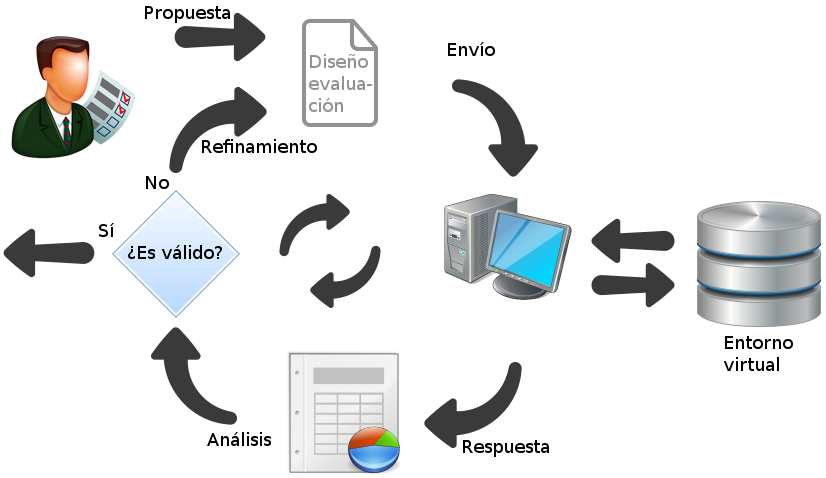
\includegraphics[scale=0.45]{CCHDiagram.png}
  \end{center}
  \caption{Diagrama del ciclo de contraste de hipótesis}
  \label{fig:CCHDiagram}
\end{figure}

\begin{enumerate}
\item \emph{Hipótesis inicial}: el profesor formula una hipótesis para la utilización de algún tipo de información de la actividad de los estudiantes en el entorno virtual para la evaluación de alguna competencia genérica (a). Por ejemplo, se considerará que un estudiante tiene un desempeño correcto de la competencia genérica de planificación y gestión del tiempo si entrega las tareas programadas por el profesor en el VLE con anterioridad a la fecha fijada para las mismas.
\item \emph{Diseño y formulación de evaluación}: el profesor diseñará un indicador para evaluar la competencia a partir de la información del registro y la implementará en la herramienta utilizada para extraer la información (b). Por ejemplo, podríamos considerar partiendo de la hipótesis anterior que un estudiante tendrá un desempeño alto en la competencia de planificación y gestión del tiempo si de las 10 tareas programadas durante el semestre al menos 9 fueron entregadas antes de la fecha fijada para las mismas, un desempeño medio si entregó entre 7 y 8 tareas antes de la fecha fijada y un desempeño bajo si entregó 6 o menos tareas antes de la fecha fijada.
\item \emph{Petición de datos}: Se enviará la petición de datos al sistema encargado de recuperar la información (c). Las herramientas y su funcionamiento serán explicadas más adelante en la sección~\ref{sec:tools}.
\item \emph{Validación de resultados}: la herramienta pondrá a disposición del profesor los indicadores requeridos (d). El profesor los analizará (e) y evaluará si son válidos para el propósito que fueron diseñados (f), si necesitan ser refinados o si hay que descartarlos. En este caso, podrá volver al segundo punto y rediseñar una nueva evaluación (g).
\end{enumerate}

\section{Características}

Con respecto a la clasificación de métodos de evaluación mostrada en la sección~\ref{sec:methods}, el método para la evaluación de competencias genéricas basado en el \emph{ciclo de contraste de hipótesis} es un método de \emph{evaluación formativo}, ya que permite mejorar el aprendizaje mientras este tiene lugar proporcionando información de manera sistemática y tan continua como el profesor desee sobre el proceso de aprendizaje.

Mientras que con respecto a la clasificación de técnicas de evaluación mostrada en la sección~\ref{sec:techniques}, la técnica empleada en este método es la de obtención de \emph{indicadores del trabajo en actividades de aprendizaje}.

El método debe cumplir una serie de requisitos que parten de los inconvenientes encontrados en la revisión de la literatura realizada en el capítulo \ref{cha:State of the Art} y que han sido resumidos en el capítulo \ref{cha:Problemas}. A continuación se describe cada uno de estos requisitos.

\paragraph*{Indicadores objetivos}

Los indicadores reflejan los datos obtenidos directamente del registro de las actividades de aprendizaje, por lo que serán objetivos per sé. No ha lugar a consideraciones personales o interpretaciones inexactas de rúbricas cómo ocurría en la autoevaluación o evaluación entre iguales, dónde dos evaluaciones de un mismo trabajo realizadas por personas diferentes podrían tener calificaciones diferentes. En el caso de los indicadores obtenidos del registro de las actividades aprendizaje, dos estudiantes que tienen los mismos datos en el registro tendrán en el mismo valor en el indicador, y ya será decisión del profesor la interpretación del indicador.

\paragraph*{Evaluación escalable}

El método para la evaluación de competencias genéricas es escalable y no supone al profesor un esfuerzo que éste no pueda abordar. El método se implementa en una herramienta que se alinea con las actividades aprendizaje, el profesor puede consultar los indicadores del registro con una simple interacción con la herramienta, esta procesa la petición y la información es devuelta en formatos que el profesor puede visionar y exportar a otras herramientas.

\paragraph*{Propósito general}

El propósito del método es obtener indicadores del registro de las actividades de aprendizaje y que estos sean utilizados para evaluar competencias genéricas. Pero no están orientados a una competencia genérica concreta, sino que es el profesor quien diseña sus actividades en el entorno virtual y el que luego obtiene los indicadores para después utilizarlos en la evaluación de la competencia genérica que considera que los estudiantes han desempeñado en dicha tarea (y que queda reflejada en los indicadores). El profesor podría incluso utilizar los indicadores para evaluar competencias específicas si lo creyese oportuno. Pero en ningún caso este método tendrá como propósito una competencia y actividad concreta como ocurría, por ejemplo, con algunos juegos serios recogidos en el estado del arte.

\paragraph*{Coste asumible}

Las herramientas que implementan el método se distribuyen como software libre, por lo que están disponibles en internet a disposición del profesor que la quiera utilizar. Además, no es necesario que el profesor tenga un perfil informático u otro específico para poder realizar las peticiones de los indicadores, ni que contrate a un equipo de expertos para obtener los indicadores. La interfaz en la que se implemente el método es usable y sencilla para que los profesores puedan utilizarla sin requerirles conocimientos técnicos, y los formatos a los que se exporta la información son figuras y documentos en formatos transportables a cualquier hoja de cálculo.

\paragraph*{Diseño de evaluaciones}

La herramienta proporciona al profesor la posibilidad de diseñar sus propias evaluaciones a partir de los indicadores. En el estado del arte nos encontramos con trabajos que obtenían sus evaluaciones a partir de los indicadores del VLE, pero éstos eran fijos. Es decir, cada competencia se evaluaba con un indicador dado. Pero podía ocurrir que el profesor no utilizase las actividades del VLE que proporcionaban dichos indicadores o que utilizase las actividades con un enfoque diferente. Con este método el profesor es quién diseña sus indicadores, y por tanto, sus evaluaciones a partir de los registros de las actividades de aprendizaje.
%  También podría ocurrir que quisiera combinar el resultado de un indicador con otro para obtener lo que él considerará un indicador válido de la competencia.

\paragraph*{Conclusiones}

En resumen, podemos decir que el método que se propone para evaluar competencias genéricas a partir de los registros de interacción de las actividades de aprendizaje se pone a disposición del profesor en forma de una herramienta informática que se conecta a la actividad de aprendizaje utilizado en la asignatura. Mediante esta herramienta, los profesores pueden diseñar evaluaciones a partir de indicadores objetivos obtenidos del VLE y aplicarlos a las competencias genéricas para las que ellos consideren que les son válidos.


%\section{Learning analytics}

%Este término ya apareció en capítulos anteriores, pero es necesario volver a traerlo y hablar más en profundidad sobre él ya que es la base del método presentado en este trabajo. El \emph{learning analytics} es la medición, recopilación, análisis y presentación de datos sobre los estudiantes, sus contextos y las interacciones que allí se generan, con el fin de comprender el proceso de aprendizaje que se está desarrollando y optimizar los entornos en los que se produce~\cite{siemens2012learning}.


\section{Implementaciones}
\label{sec:tools}

Hay diversos entornos en los que se pueden desarrollar actividades de aprendizaje. Para la implementación del método se seleccionaron tres entornos diferentes: el primer entorno fue un wiki, entorno de trabajo online donde los usuarios crean y editan el contenido de forma colaborativa; el segundo fue un VLE, entorno de aprendizaje virtual donde se alojan cursos virtuales constituidos por una miríada de herramientas; y el tercero un mundo virtual, donde los estudiantes afrontan situaciones de la vida real en un entorno de simulación virtual.

En las próximas secciones se describirán cada una de las herramientas implementadas para aplicar el método en cada uno de los entornos virtuales: AssessMediaWiki para wikis, EvalCourse para VLEs y EvalSim para mundos virtuales.

%------------------------------------------------
\subsection{Wikis}

El uso educacional de los wikis para las experiencias de trabajo colaborativo está en auge debido a las numerosas ventajas que aporta sobre los modelos tradicionales~\cite{elgort2008wiki}. Algunas de las ventajas sobre los medios tradicionales, ya sean en formato impreso o en documentos digitales, es que éstos no llevan un registro de ediciones, no permiten la colaboración distribuida y asíncrona y no pueden ser monitorizados por el profesor mientras los estudiantes completan el trabajo.

Para evaluar el trabajo final de un grupo de estudiantes en una página del wiki nos bastaría con leer la última versión de dicha página, como hacíamos con los métodos tradicionales. Pero una de las características más interesantes de los wikis es que no sólo almacenan la información de la versión final de cada documento, sino que también almacenan todas las versiones intermedias creadas como resultado de las contribuciones hechas por cada usuario~\cite{trentin2009using}. Esto lo consigue manteniendo un registro con las diferencias entre las ediciones consecutivas de las páginas, registro que se podría utilizar para la obtención de indicadores de diferentes competencias~\cite{ortega2011new}. Las páginas creadas de manera colaborativa podrían ser evaluadas considerando la contribución de cada autor y las dinámicas de grupo en la creación de la página en tiempo real. Por desgracia, realizar una evaluación detallada de cada contribución realizada en el wiki es imposible de abordar cuando hay muchos usuarios y éstos participan activamente.

En un trabajo anterior se utilizó \emph{StatMediaWiki} (SMW)~\footnote{http://statmediawiki.forja.rediris.es/}, una herramienta que proporciona al profesor información cuantitativa sobre la distribución del trabajo de los estudiantes en las páginas del wiki, es decir, qué parte del trabajo realizado en una página del wiki corresponde a cada estudiante. A partir de esa información cuantitativa se evaluó la distribución del trabajo, el trabajo en equipo y el liderazgo. Sin embargo, el aspecto cualitativo quedó fuera, ya que el experimento sólo consideró el número, el momento y el tamaño de las contribuciones~\cite{palomo2014assessment}.

Para completar el análisis cuantitativo proporcionado por SMW con un análisis cualitativo se desarrolló \emph{AssessMediaWiki} (AMW)~\footnote{http://assessmediawiki.forja.rediris.es}. AMW es una herramienta para realizar una evaluación escalable y cualitativa del trabajo realizado en el wiki mediante procedimientos de autoevaluación, evaluación entre iguales y evaluación del profesor.

\subsubsection{AssessMediaWiki (AMW)}

La aplicación creada para poner en práctica este método es AMW. AMW es una aplicación web de código abierto que, al conectarse a una instalación MediaWiki, proporciona procedimientos de autoevaluación, evaluación entre iguales y evaluación del profesor, a la vez que mantiene información sobre esas evaluaciones. AMW pone a disposición de los estudiantes una rúbrica previamente definida por el profesor para que realicen la evaluación (figura\ref{fig:AmwRubrica}). 

\begin{figure}
  \begin{center}
    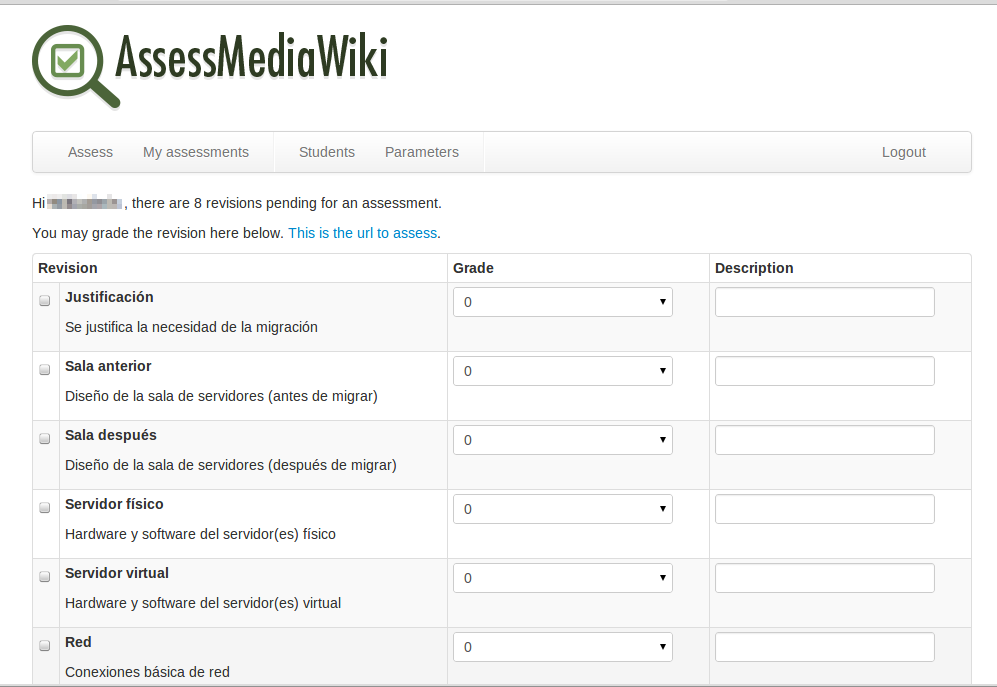
\includegraphics[scale=0.3]{AmwRubrica.png}
  \end{center}
  \caption{Rúbrica de AMW}
  \label{fig:AmwRubrica}
\end{figure}

AMW implementa dos roles de usuario distintos: supervisores y estudiantes. Los estudiantes pueden elegir entre distintas opciones: evaluar una revisión, comprobar sus propias aportaciones evaluadas y verificar las evaluaciones ya enviadas. Por otro lado, los supervisores tienen un mayor número de opciones, como definir la rúbrica que los estudiantes deberán completar al realizar sus evaluaciones, modificar los parámetros de los programas o vigilar las evaluaciones que los alumnos vayan haciendo. AMW implementa un función de selección parcialmente aleatoria. Cuando un estudiante va a realizar una evaluación, el sistema elige automáticamente una de entre el 30\percentage más significativa que aún no ha sido evaluada.

Al revisar sus evaluaciones, los estudiantes puede revisar las notas recibidas y sus justificaciones, así como ver a qué contribución en particular se refiere (figura~\ref{fig:AmwFormative}). Si el estudiante no está de acuerdo con la calificación puede replicar utilizando para ello una réplica similar a la que se utilizó en su evaluación, indicando las calificaciones que considera que merece y sus correspondientes justificaciones. Después el profesor revisará la disputa y pondrá la nota definitiva.

\begin{figure}
  \begin{center}
    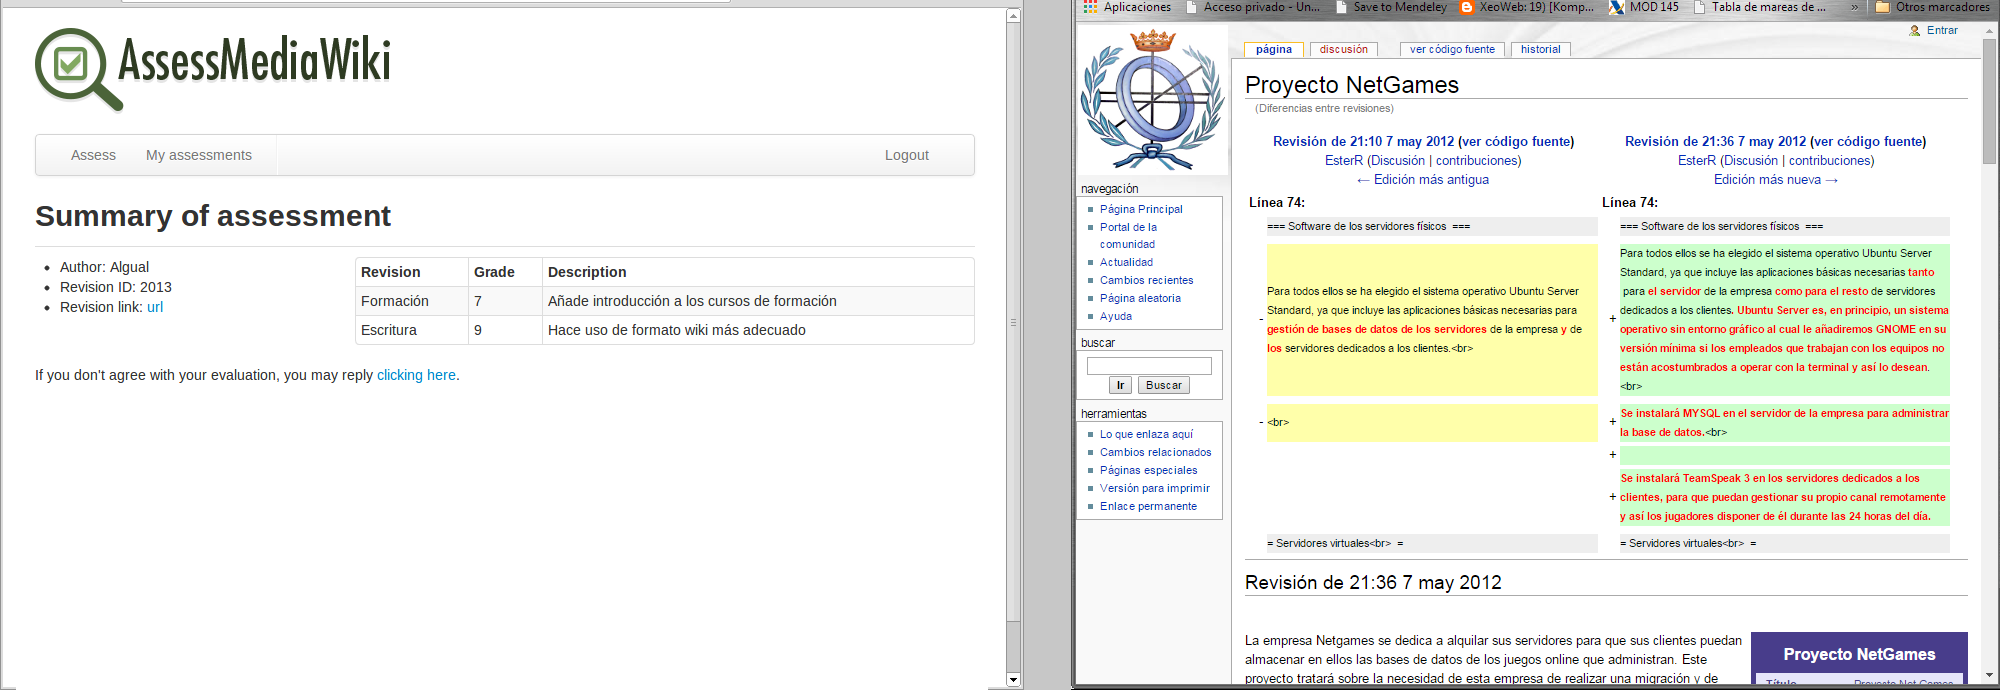
\includegraphics[scale=0.19]{AmwFormative.png}
  \end{center}
  \caption{Ejemplo de retroalimentación formativa y la contribución de wiki evaluada}
  \label{fig:AmwFormative}
\end{figure}

\subsubsection{Método}

El método para la evaluación del trabajo y las competencias desempeñadas en el wiki consta de dos partes: una primera parte en la que lo que se evalúa es el trabajo del wiki, basada en procedimientos de autoevaluación, evaluación entre iguales y evaluación del profesor; y una segunda parte en la que se evalúan las competencias genéricas y es donde se pone en práctica el \emph{ciclo de contraste de hipótesis}.

\paragraph{Evaluación del trabajo en el wiki}

El método para la evaluación del trabajo en el wiki se divide también en tres fases: una primera fase en la que los estudiantes realizan sus trabajos en las páginas del wiki, una segunda fase de evaluación y una tercera fase de revisión del profesor. En la figura~\ref{fig:AmwDiagram} puede verse un diagrama de flujo de trabajo que muestra cada una de las fases del método de evaluación realizado sobre una página del wiki en la que participan varios estudiantes y el profesor. A continuación se describen cada una de estas fases.

\begin{figure}
  \begin{center}
    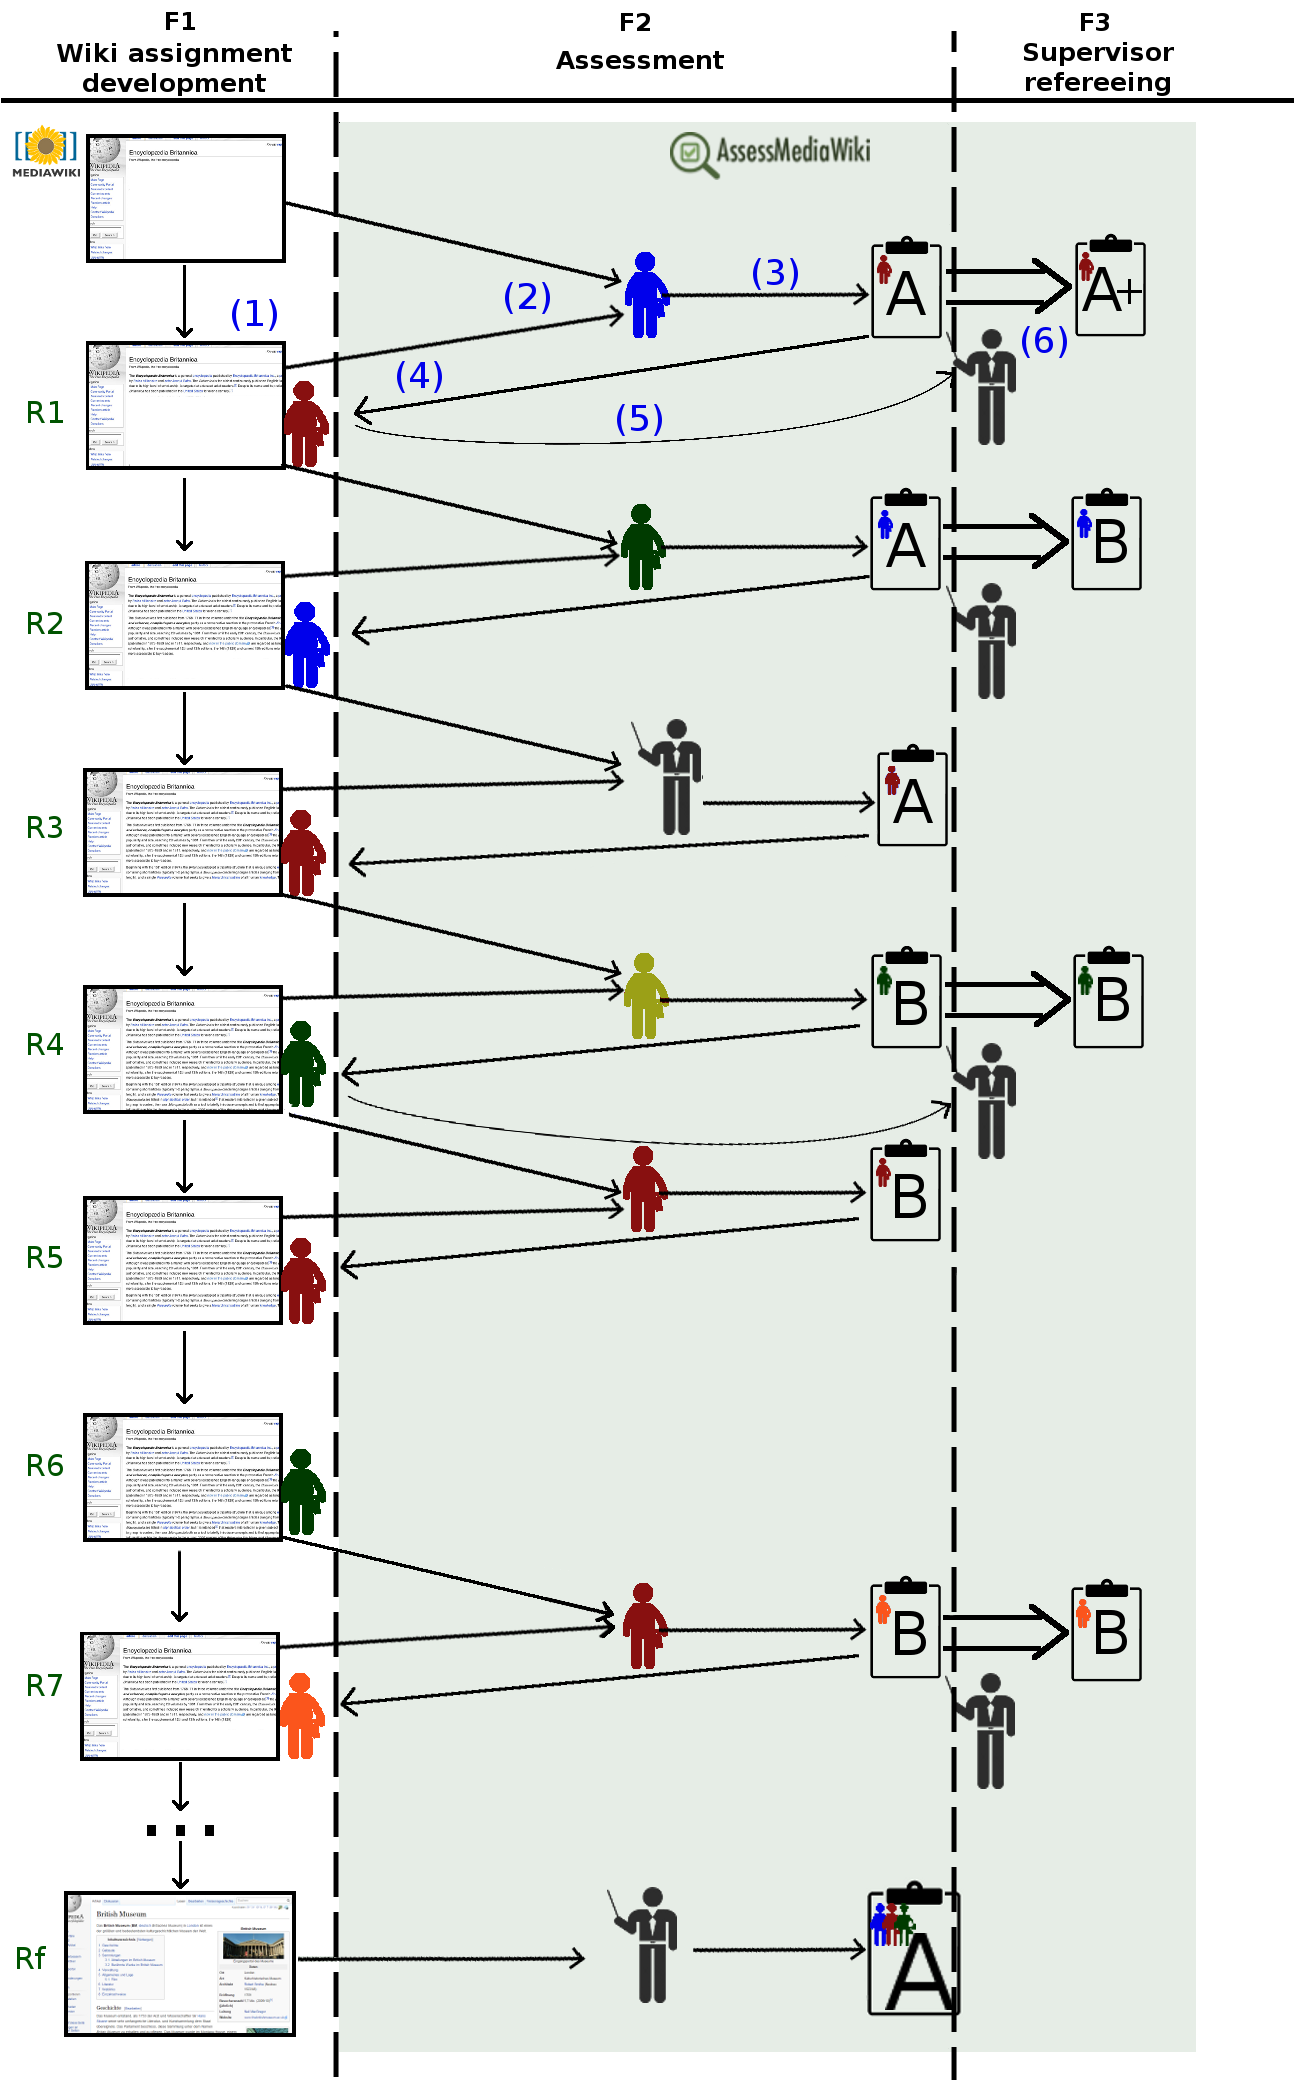
\includegraphics[scale=0.28]{AmwDiagram.png}
  \end{center}
  \caption{Ejemplo de flujo de trabajo para la evaluación cualitativa del wiki utilizando AMW}
  \label{fig:AmwDiagram}
\end{figure}

\paragraph*{Desarrollo del trabajo en el wiki}

Esta fase se representa en la columna de la izquierda de la figura~\ref{fig:AmwDiagram}, y es en la que los estudiantes realizan el trabajo en las páginas del wiki. Normalmente, cada grupo de estudiantes tendrá que desarrollar su trabajos en una página del wiki. En la zona más alta de la columna se representa el comienzo del trabajo con una página en blanco. El autor de cada contribución se muestra con una figura de color junto a la misma. Para comenzar, el usuario de color rojo crea una página vacía (\emph{R1}). Después, el usuario azul añade contenido a la página (\emph{R2}). En tercer lugar, el usuario rojo modifica de nuevo la página añadiendo texto a la versión dejada anteriormente por el usuario azul (\emph{R3}) y así sucesivamente. Esta fase termina cuando llega la fecha marcada por el profesor para que los trabajos estén finalizados (\emph{Rf} es la versión final de la página).

Puede verse que, aunque los estudiantes responsables de la página de ejemplo del wiki fuesen el rojo, el azul y el verde, otros estudiantes, como el naranja en la revisión séptima, podrían contribuir a la página del wiki. En ese caso, los miembros del grupo y responsables de la página deben decidir si la contribución debe conservarse o no.

\paragraph*{Evaluación}

Esta fase se muestra en la columna central y comprende las siguientes actividades:

\begin{itemize}
\item \emph{Autoevaluación, evaluación entre iguales y evaluación del profesor}. Las contribuciones a ser evaluadas se asignan a los estudiantes.  Cada contribución es la diferencia entre dos revisiones consecutivas de una página del wiki. El estudiante encargado de evaluar dicha contribución se representa en el gráfico como un usuario coloreado que recibe dos flechas de las revisiones, una de la revisión anterior a la contribución y otra de la revisión que incorpora ya la contribución. Para la evaluación los estudiantes utilizan una rúbrica definida por el profesor. Cada contribución sólo se refiere a una contribución atómica de las realizadas a una página del wiki por un único estudiante, por lo que dicha contribución podría ser utilizada como un indicador de la contribución al wiki de dicho estudiante. El estudiante que realizó cada contribución se representa con una figura pegada a la revisión de la página en cada momento.
Por ejemplo, en la primera evaluación, se asigna la contribución realizada a la página del wiki por el estudiante rojo (\emph{1}) al estudiante azul. El estudiante azul comprueba ambas versiones para ver las diferencias entre ambas versiones (\emph{2}) y realiza la evaluación completando la rúbrica proporcionada por el profesor (\emph{3}).
Cabe destacar también otras situaciones interesante. En la versión \emph{R5} de la página vemos como se realiza una autoevaluación, ya que el estudiante rojo, autor de la versión, es el mismo que tiene que evaluar su contribución. Vemos también que en \emph{R3} es el profesor el que realiza la evaluación de la contribución del estudiante rojo. Esto puede deberse a que el estudiante manualmente detecta una contribución que considera oportuno evaluar o a que, utilizando la herramienta SMW, detecta un comportamiento extraño en el wiki y quiere contrastar la situación. 
Puede verse también que hay contribuciones que no reciben evaluación alguna, como ocurre con \emph{R6}. Está claro que sería deseable que todas las contribuciones significativas fueran evaluadas, pero no es escalable.
\item \emph{Revisión de las evaluaciones recibidas}. Los estudiantes pueden revisar las evaluaciones recibidas. Ellos pueden no sólo ver las notas que han recibido con las justificaciones y comentarios que añadieron sus evaluadores, sino también el enlace a la contribución. De esta forma, los estudiantes evaluados reciben una retroalimentación formativa. En la primera de las evaluaciones del diagrama de ejemplo puede verse como el estudiante rojo puede ver su evaluación (\emph{4}).
\item \emph{Réplica}. Si el estudiante evaluado no está de acuerdo con la evaluación recibida tiene la opción de replicarla justificando el motivo de dicha réplica. En el diagrama de ejemplo puede verse como el estudiante rojo considera injusta su evaluación y realiza una réplica (\emph{5}). El profesor deberá resolver la réplica en la siguiente etapa.
\item \emph{Evaluación final del wiki}. El profesor evalúa la versión final de la página del wiki desarrollada por cada grupo de estudiantes. Esta evaluación es necesaria ya que el objetivo principal de la tarea es que los estudiantes realicen un buen trabajo en una página del wiki. Como cualquier otra tarea, deberá ser evaluada por el profesor conforme al programa de estudios. Además, algunos de los criterios de evaluación sólo pueden ser evaluados en la versión final de la página, como por ejemplo, la coherencia del texto. De esta forma, aquellas contribuciones del wiki descartadas por la función de selección serán ahora implícitamente evaluadas ya que están integradas en el entregable final. Puede verse la evaluación al final del diagrama de ejemplo (\emph{Rf}), y cómo afecta al grupo de estudiantes completo.
\end{itemize}

El diagrama no recoge algunas situaciones que también podrían darse. Por ejemplo, alguna contribución podría ser evaluada por más de un usuario, ya fuera otro estudiante o el profesor. También, para simplificar, el diagrama sólo muestra una calificación para la contribución (A, A+, B, ... etc.), pero las evaluaciones son multidimensionales.

Un componente interesante de nuestro algoritmo es qué contribución wiki podrá ser asignada a cada estudiante para su evaluación. Es lo que llamamos \emph{función de selección}, y tiene varios aspectos a tener en cuenta:

\begin{itemize}
\item \emph{¿Debería cierta contribución en el wiki ser evaluada por más de un estudiante?} En realidad, tener varias evaluaciones de estudiantes diferentes sobre una misma contribución podría ser interesante para perfeccionar su evaluación y podría proporcionar información al profesor para evaluar no sólo al estudiante autor de la contribución, sino también a los evaluadores. De hecho, el número de contribuciones a ser evaluadas es dependiente del objetivo del experimento y su configuración. Cuánto más grande sea el experimento, más contribuciones susceptibles de ser evaluadas tendrá. Sin embargo, el número de evaluaciones que un estudiante puede realizar es limitado (para que siga siendo formativo). Por lo que cada evaluación adicional a la misma contribución provocará que otras contribuciones sean más pobremente evaluadas o que no lo sean.
\item \emph{¿Qué contribuciones deberían ser evaluadas?} La importancia de evaluar cada contribución puede variar. Por ejemplo, evaluar al menos una mínima cantidad de contribuciones por cada estudiante, página o categoría sería interesante. Pero algunas contribuciones que añadan ciertas características al trabajo pueden ser relevantes o informativas sobre el trabajo realizado por un estudiante. Por ejemplo, aunque las contribuciones que añadan gran cantidad de texto suelan ser más interesantes que las contribuciones pequeñas, una contribución pequeña puede ir relacionada con el cambio de sentido de alguna frase o párrafo. De cualquier forma, un estudiante puede solicitar que una contribución en particular sea evaluada, aunque ésta quede fuera de la función de selección.
\item \emph{¿Quién evalúa cada contribución?} Depende de la importancia que se quiera dar a la autoevaluación, la evaluación del compañero y la del profesor. De nuevo, se debería balancear el esfuerzo requerido y el detalle a exigir en las evaluaciones.
\end{itemize}


\paragraph*{Revisión del profesor}

En esta última columna se representan dos actividades que corresponden al profesor:

\begin{itemize}
\item Resolución de las réplicas: el profesor revisa las réplicas indicando si proceden o no. En caso de que procedan, modifica la calificación. En el diagrama se puede ver como en la primera contribución, el estudiante rojo realiza una réplica (\emph{5}) sobre la evaluación reciba por el usuario azul (\emph{3}). El profesor revisa la réplica, la considera apropiada y modifica la calificación (\emph{6}). En un segundo ejemplo, en la evaluación realizada por el estudiante de color amarillo sobre la contribución realizada por el usuario de color verde puede verse como el profesor no acepta la réplica realizada por este último, y mantiene la calificación otorgada inicialmente por el estudiante amarillo.
\item Revisión de evaluaciones no replicadas: el profesor puede revisar aleatoriamente otras evaluaciones realizadas por los estudiantes que no hayan sido replicadas. En el diagrama puede verse como en el profesor revisa las evaluaciones realizadas sobre las contribuciones representadas en \emph{R2} y en \emph{R7}, disminuyendo la calificación de la primera y manteniendo la segunda.
\end{itemize}

\paragraph{Evaluación de competencias genéricas}

El método para la evaluación de competencias genéricas se basa en el \emph{ciclo de contraste de hipótesis}. En la figura~\ref{fig:AmwDiagram2} puede verse la descripción del método. Esta evaluación se puede llevar a cabo durante o después de que los estudiantes hayan realizado su trabajo en el wiki y sus evaluaciones con AMW. Evidentemente, cuánto más avanzado esté el trabajo más datos habrá para analizar. 

El ciclo comienza con el diseño de un indicador por parte del profesor que plasmará en una hoja de cálculo a partir de los datos que recibirá de las evaluaciones (a). A continuación, el profesor realiza la petición a AMW que le proporcionará los datos (b). AMW consulta y procesa los datos en las bases de datos de MediaWiki y AMW (c) y se los envía al profesor (d). El profesor los integra en la hoja de cálculo previamente diseñada y los analiza (e). Si son válidos para la evaluación finaliza el proceso (f). Por el contrario, si necesitan algún tipo de refinamiento el profesor puede rediseñar la evaluación (g) y hacer una nueva petición.

\begin{figure}
  \begin{center}
    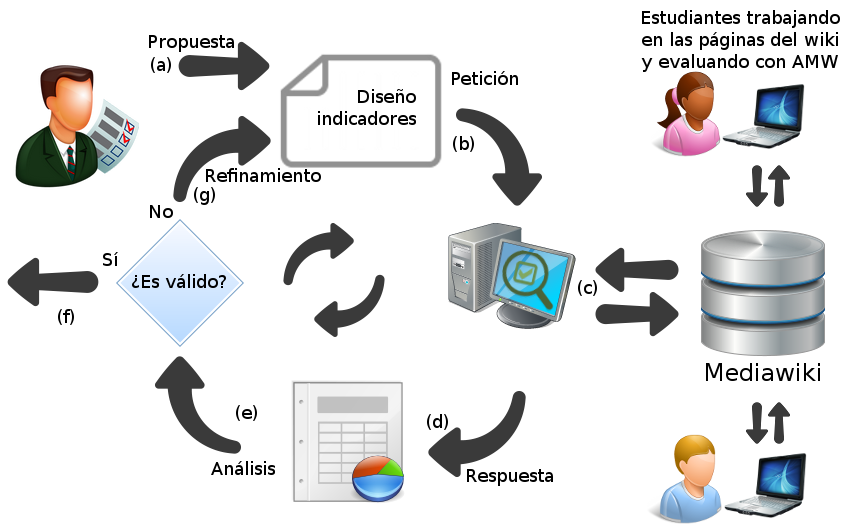
\includegraphics[scale=0.45]{AmwDiagram2.png}
  \end{center}
  \caption{Ciclo de contraste de hipótesis para la evaluación en wikis}
  \label{fig:AmwDiagram2}
\end{figure}

\subsubsection{Indicadores}

Los indicadores que se mencionan en este punto han sido utilizados en los estudios de caso realizados para este trabajo, pero como se ha mencionado desde un primer momento, este método proporciona indicadores y es el profesor el que los utilizará para evaluar las competencias genéricas que considere oportunas.

\paragraph*{Trabajo en equipo}
El indicador considerado para el trabajo en equipo es el \emph{ratio de miembros del equipo que trabajaron en un mismo criterio.} La rúbrica que utilizan los estudiantes para evaluar se compone de un conjunto de criterios. Cada criterio puede hacer referencia a una parte del trabajo. En todas las ediciones de un wiki no se trabajan en las mismas partes del trabajo, por lo que al ser evaluado, un estudiante puede tener nota en unos criterios y no tenerla en otros. Si más de un estudiante ha trabajado en la misma parte de una página wiki y su aportación ha sido significativa, tendrán nota en dicho criterio. Por tanto, partiendo de la cantidad de criterios que tiene un trabajo y del ratio de miembros del equipo que ha trabajado en cada criterio tendremos un indicador del trabajo en equipo.

\paragraph*{Comunicación y aplicación del conocimiento}
El indicador considerado para la comunicación y la aplicación del conocimiento es la \emph{media de las notas recibidas por todos los miembros del grupo}. Este indicador mide la incidencia que tuvieron las contribuciones realizadas en el éxito del proyecto. Una calificación pobre en una contribución puede significar  que alguna contribución wiki obtuvo una buena nota en un cierto criterio de la rúbrica pero una mala nota en el otro (el autor de la contribución soluciona un problema y crea uno nuevo). Probablemente, esto se debió a una mala comunicación entre los miembros del equipo o poco compromiso de un determinado alumno en el objetivo global del grupo. 

\paragraph*{Mantener la calidad del trabajo producido}
El indicador considerado para el mantenimiento de la calidad del trabajo producido es la \emph{media de las notas que cada estudiante individualmente recibió}. Unas calificaciones altas en las evaluaciones recibidas pueden significar que el trabajo que el estudiante está produciendo es de calidad. Si el estudiante produjese mucho contenido, pero este no fuese de calidad, las calificaciones no serían buenas. Es decir, sus calificaciones están teniendo en cuenta el aspecto cualitativo del trabajo y por tanto una nota alta significaría un trabajo de calidad.

\paragraph*{Capacidad crítica}
El indicador considerado para la capacidad crítica es el \emph{número de evaluaciones que el estudiante realizó con respecto al número de dichas evaluaciones cuya nota fue modificada por el profesor}. Este indicador mide la competencia de un estudiante para evaluar el trabajo hecho por otros. Si recibiera un número fijado de réplicas en sus revisiones y estas fueran revisadas por el profesor modificando las calificaciones, podríamos considerar que dicho alumno no ha desempeñado bien dicha competencia.

En la tabla~\ref{tab:ResumenIndicadoresCualiCuanti} puede verse una comparación entre los indicadores considerados a partir de la evaluación cualitativa que se realizaría con AMW y los que se obtienen a partir de la evaluación cuantitativa realizada con SMW.

\begin{table}
  \begin{center}
  \begin{tabular}{| m{3.2cm} | m{4.9cm} | m{5.1cm} |}
    \hline 
    \multirow{2}{*}{COMPETENCIAS}  & INDICADORES  & INDICADORES  \\
      &  CUALITATIVOS  &  CUANTITATIVOS \\
    \hline
    \hline
    Trabajo en equipo  & Ratio de miembros del equipo que trabajaron en un mismo criterio  & Ratio de miembros del equipo que contribuyeron a una misma página del wiki en las páginas de su proyecto \\
    \hline
    Comunicación y aplicación del conocimiento  & Media de las notas recibidas por todos los miembros del grupo  & Porcentaje de miembros del equipo que contribuyeron al menos a un 20\percentage del trabajo realizado \\
    \hline
    Mantener la calidad del trabajo producido  & Media de las notas que cada estudiante individualmente recibió  & Contribución individual en bytes \\
    \hline
    Capacidad crítica  & Número de evaluaciones que el estudiante realizó con respecto al número de dichas evaluaciones cuya nota fue modificada por el profesor  & No considerada \\
    \hline
  \end{tabular}
\end{center}
\caption{Resumen de las competencias evaluadas para cada tipo de indicador}
\label{tab:ResumenIndicadoresCualiCuanti}
\end{table} 

%\subsubsection{Ejemplo de uso}

%El ejemplo de uso podrá verse en el estudio de caso que se muestra en el siguiente capítulo.
%\subsubsection{Publicación}

%Un trabajo con AMW fue publicado en SPDECE 2012~\cite{Balderas:2012}.
% La evaluación de las 3 herramientas se corresponde al capítulo siguiente.

%-----------------------------------------------------------------------------------------------------------------------------------------------
\subsection{VLE}

En esta segunda propuesta el método se aplica a los cursos virtuales. El VLE es el núcleo de los cursos virtuales, donde los profesores ponen el material a disposición de los estudiantes y donde los estudiantes pueden fácilmente acceder a ellos; donde tanto los profesores como los estudiantes se pueden comunicar entre ellos de manera síncrona y asíncrona; y donde los estudiantes gestionan sus proyectos en equipo mientras dialogan entre ellos. Gracias a la gran cantidad de información que genera la actividad de los estudiantes y que queda registrada en el VLE, los investigadores de diferentes áreas han colaborado para extraerlos, realizar minería de datos y utilizarlos para mejorar el aprendizaje~\cite{park2015development}.

Además, en algunos de los trabajo recopilados en el estado del arte mostrado en el capítulo~\ref{cha:State of the Art}, se confirma la relación entre la interacción que llevan a cabo los estudiantes en el VLE y su rendimiento en el desempeño de varias competencias genéricas~\cite{fidalgo:2015,rayon2014web}. 

Por tanto, y tal y cómo se mostrará a continuación, en esta propuesta se utilizarán indicadores obtenidos de la interacción de los estudiantes en el VLE para el diseño de evaluaciones de competencias genéricas dentro del  \emph{ciclo de contraste de hipótesis}.


\subsubsection{SASQL y EvalCourse}

Para diseñar evaluaciones a partir de los indicadores del VLE se crea un lenguaje especifico de dominio (DSL, del inglés \emph{domain-specific language})~\cite{vanDeursen:2000}: \emph{Simple Assessment-Specific Query Language} (SASQL). Es un lenguaje formal para la ejecución automática de consultas simples escritas utilizando un lenguaje específico de evaluación. SASQL tiene un sintaxis simple, orientada a la evaluación de competencias genéricas~\cite{Balderas:2013}. De esta forma, los profesores pueden fácilmente obtener indicadores almacenados de la actividad en el VLE sin requerir conocimientos técnicos en bases de datos o programación informática.

También se implementa \emph{EvalCourse}, una herramienta informática que ejecuta instrucciones escritas en SASQL, proporcionando como resultado los indicadores solicitados. EvalCourse se comunica con el VLE para extraer la información del registro de actividad. EvalCourse\footnote{https://www.assembla.com/spaces/evalcourse} está basado en el IDE de la plataforma Eclipse, fue implementado utilizando Xtext~\cite{eysholdt2010xtext} dentro del Eclipse Modeling Framework y está disponible como software libre bajo licencia GNU GPL.

El desarrollo de EvalCourse y SASQL se basa en los principios y técnicas de la ingeniería dirigida por modelos (MDE, del inglés Model-Driven Engineering). Este enfoque promueve la construcción de artefactos software de un modo flexible y rápido mediante el desarrollo de modelos y sus transformaciones. Nuestro DSL se define en términos de su sintaxis abstracta o metamodelo, su sintaxis concreta y un conjunto de plantillas para la transformación de modelos de consulta en código ejecutable dependiente del VLE.

\begin{figure}
  \begin{center}
    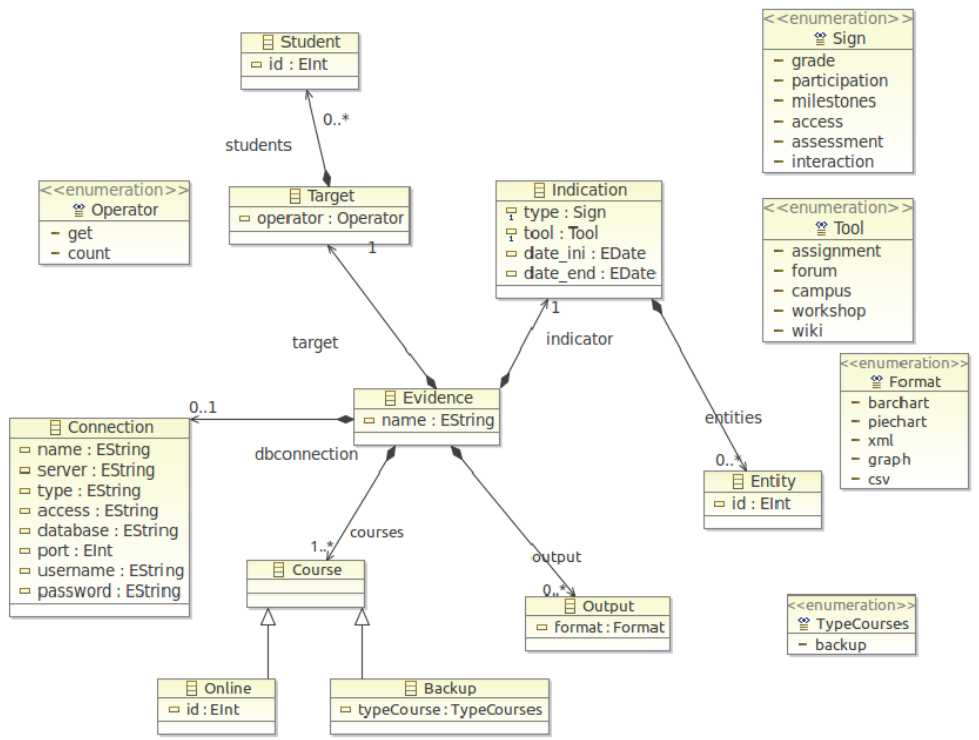
\includegraphics[scale=0.4]{EvcMetamodel.png}
  \end{center}
  \caption{Metamodelo de SASQL}
  \label{fig:EvcMetamodel}
\end{figure}

El metamodelo de EvalCourse puede verse en la figura~\ref{fig:EvcMetamodel}. La entidad principal es el indicador o evidencia (\emph{evidence}). Esta evidencia se aplicará a una herramienta (\emph{tool}) que puede ser tarea (\emph{assignment}), foro (\emph{forum}), campus (\emph{campus}), taller (\emph{workshop}) o wiki (\emph{wiki}), en las que se observará un indicio (\emph{sign}), que puede ser participación (\emph{participation}), entregas (\emph{milestones}), accesos (\emph{access}), evaluaciones (\emph{assessment}), interacción (\emph{interaction}) o calificación (\emph{grade}). Además, puede actuarse sobre una actividad específica (\emph{entity}) o sobre todas las actividades de un tipo que se han dado en el VLE. La conexión a la base de datos del curso se declara en la entidad \emph{connection}. 

La sintaxis de SASQL puede verse en la consulta~\ref{code:sasqlSintax}. En la primera línea se comienza con la palabra reservada \emph{Evidence} seguida del nombre que se dará al indicador. Ese nombre será el que tengan todos los ficheros de salida. En la segunda línea se escriben los términos obligatorios \emph{get students}. En la tercera, se indica qué indicio se quiere extraer (\emph{show milestones | participation | access | interaction | assessment | grade}). En la consulta, la tercera línea se divide en dos (tercera y cuarta) para que puedan ser visualizadas todas las opciones. En la quinta, se indica sobre qué herramienta se quiere obtener el indicio (\emph{ in assignment | forum | campus | workshop | wiki [list of ids]}). También la quinta línea se divide en dos (quinta y sexta). En la séptima línea, que es opcional, se indica el rango de fechas sobre los que se extraerá la información. Y por último, en la octava se especifica si la conexión se realizará directamente a la base de datos o sobre una copia de seguridad almacenada en un fichero.

\begin{lstlisting}[caption=Sintaxis de SASQL (las palabras reservadas se muestran resaltadas),label=code:sasqlSintax,numbers=left, captionpos=b, morekeywords={Evidence,get, students, show, milestones, participation, access, in, assignment, forum, campus, wiki, between, and, workshop, interaction, assessment, grade, from, course, backup}]
Evidence indicator_name:
 get students 
 show milestones | participation | access 
	| interaction | assessment | grade
 in assignment | forum | campus | workshop 
	| wiki [list of ids]
 between YYYY-MM-DD and YYYY-MM-DD
 from course id | backup.
\end{lstlisting}

El objetivo es que EvalCourse pueda ser utilizado para cualquier VLE, pero esta primera versión ha sido implementada para funcionar en Moodle~\footnote{https://moodle.org/}. Moodle es un sistema de gestión de aprendizaje de código abierto con más de 64.000 sitios registrados~\footnote{https://moodle.net/stats}, y que además es el que se utiliza en la Universidad de Cádiz.

\subsubsection{Método}

Para evaluar las competencias genéricas el profesor deberá definir los indicadores que serán extraídos de la actividad de cada estudiante en el VLE. Ilustraremos el método a partir de un ejemplo de uso de EvalCourse y su ejecución con los foros del VLE. Los foros suelen ser una de las herramientas incorporadas por los VLEs para la interacción entre los estudiantes. Es evidente que la comunicación oral es una manera muy rica de comunicarse, que proporciona múltiples signos no verbales como las expresiones faciales o el tono de voz. En contraste, las comunicaciones escritas proporcionan otras ventajas. Una de las más importantes para la educación es que el estudiante dispone de un tiempo para la reflexión. Por esta razón, podría preferirse la comunicación escrita a la oral cuando se busca un aprendizaje cognitivo~\cite{garrison1999critical}.

La obtención de indicadores se basará en el \emph{ciclo de contraste de hipótesis}(figura~\ref{fig:EVCDiagram}). En primer lugar, es necesario que los estudiantes hayan interactuado en el VLE, de manera que su actividad haya quedado registrada. Entonces, el profesor propone un diseño de evaluación mediante una consulta SASQL (a) y envía esta consulta a EvalCourse (b). EvalCourse procesa la consulta, realiza la petición a la base de datos y recoge los datos (c). Entonces EvalCourse devuelve los resultados (d). El profesor analiza los resultados conforme a su propuesta de evaluación de competencias (e), terminando el proceso si éstos son válidos para él (f). Por el contrario, si los resultados no son válidos como indicadores de la competencia, entonces el profesor podrá rediseñar la evaluación (g). En cualquier caso, el profesor podrá reutilizar el diseño cuántas veces sea necesaria a lo largo del curso y monitorizar la evolución de los indicadores de cada estudiante.

\begin{figure}
  \begin{center}
    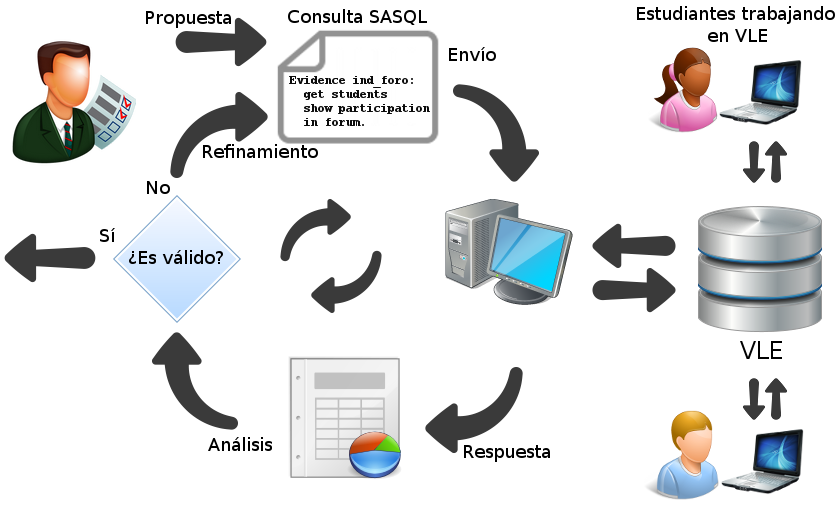
\includegraphics[scale=0.45]{EvcDiagram.png}
  \end{center}
  \caption{Ciclo de contraste de hipótesis utilizando EvalCourse}
  \label{fig:EVCDiagram}
\end{figure}

\paragraph*{Ejemplo de uso}

En este ejemplo, el profesor pretende obtener indicadores del uso del foro para evaluar la competencia genérica de las habilidades interpersonales. Durante el curso, los estudiantes interactuarán en el foro conforme a las instrucciones proporcionadas por el profesor. Cuando lo desee, el profesor podrá utilizar EvalCourse para obtener los indicadores.

% Estos indicadores deben ser publicados para que los estudiantes sepan cómo serán evaluados % FRASE ELIMINADA DEL MEDIO DEL PÁRRAFO ANTERIOR

El profesor considera que podría diseñar un indicador válido a partir del número de mensajes que ha escrito cada estudiante en un periodo de tiempo particular y plantea la siguiente hipótesis: \emph{se considerará que un estudiante ha desempeñado satisfactoriamente la competencia genérica de las habilidades interpersonales si ha escrito al menos dos mensajes en el foro}. Para ello se diseña la consulta~\ref{code:sasqlejemplo1}. EvalCourse procesa la consulta y devuelve los resultados que se pueden ver en la tabla~\ref{tab:EvalCourseEj1}.

\begin{lstlisting}[caption=Participación en el foro en un periodo concreto de tiempo ,label=code:sasqlejemplo1,numbers=left, captionpos=b, morekeywords={Evidence,get, students, show, milestones, participation, access, in, assignment, forum, campus, workshop, interaction, between, and}]
Evidence participacion_foro: 
	get students
	show participation
	in forum between 2015-10-21 and 2015-10-27.
\end{lstlisting}

\begin{table}
	\centering
	\caption{Información sobre la participación en el foro de los estudiantes en un periodo concreto de tiempo}
	\label{tab:EvalCourseEj1}
	\begin{tabular}{|l|l|c|c|c|c|c|}
		\hline
		id & username & Debate-starter & Debate-participation & Total \\
		\hline
		\hline
		1 & student1 & 1 & 2 & 3  \\
		\hline
		2 & student2 & 0 & 4 & 4  \\
		\hline
		3 & student3 & 0 & 1 & 1  \\
		\hline
		4 & student4 & 1 & 2 & 3  \\
		\hline
		5 & student5 & 0 & 2 & 2  \\
		\hline
	\end{tabular}
\end{table}

A la vista de los resultados, y en base a la hipótesis inicial, se podría decir que todos los estudiantes menos el 3 (\emph{student3}) habrían desempeñado correctamente la competencia. Sin embargo, el profesor considera que esta primera aproximación es un poco pobre y decide completar su hipótesis de la siguiente manera: \emph{se considerará que un estudiante ha desempeñado satisfactoriamente la competencia genérica de las habilidades interpersonales si ha escrito al menos dos mensajes en el foro y ha interactuado con más de un compañero}. Para ello escribe la consulta~\ref{code:sasqlejemplo2}. 

\begin{lstlisting}[caption=Interacción en el foro en un periodo de tiempo ,label=code:sasqlejemplo2,numbers=left, captionpos=b, morekeywords={Evidence,get, students, show, milestones, participation, access, in, assignment, forum, campus, workshop, interaction, between, and}]
Evidence interacciones_foro: 
	get students
	show interaction
	in forum between 2013-10-21 and 2013-10-27.
\end{lstlisting}

Además del listado con las interacciones, EvalCourse proporciona varias figuras con la representación de la información. Para esta última consulta se devuelve un grafo para una mejor visualización de las interacciones (figura~\ref{fig:EvalCourseInteraccionForo}). A tenor de los resultados vemos que sólo dos de los estudiantes cumplen la segunda hipótesis (\emph{student2} y \emph{student4}). 

\begin{figure}
	\centering
	\includegraphics[width=6cm]{{EvalCourseInteraccionForo.png}}
	\caption{Interacción en el foro en un periodo de tiempo.}
	\label{fig:EvalCourseInteraccionForo}
\end{figure}

De esta manera, el profesor irá redefiniendo sus hipótesis hasta dar con los indicadores que a su juicio satisfagan la evaluación de la competencia genérica.

\subsubsection{Indicadores}

En este apartado se muestra una propuesta de uso de indicadores obtenidos mediante EvalCourse para la evaluación de competencias genéricas~\cite{Balderas:2015}. Pero al igual que ocurre con el resto de herramientas, estos indicadores podrían ser válidos para unos profesores y no serlos para otros, así como que habrá otras muchas formas de combinar la información del registro para obtener indicadores válidos para otras competencias genéricas.

\paragraph*{Habilidades interpersonales}
Para la evaluación de esta competencia genérica se propone utilizar la participación en el foro. Al crear grupos de trabajo en el VLE se puede crear un foro para cada grupo. Durante el curso se fomenta que los estudiantes intervengan en dichos foros para comunicarse entre los miembros del equipo y dejar constancia de los mensajes de cara al profesor. Por tanto, si no utilizan el foro, los estudiantes no tienen calificación en esta competencia. Por ejemplo, podría fijarse que un estudiante que tuviera tres o más intervenciones en el foro tendría una evaluación positiva en la competencia.

\paragraph*{Liderazgo}
Para evaluar el liderazgo de los estudiantes se proponen también los foros creados para la comunicación de los equipos de trabajo. Para ello se podría considerar la cantidad de debates que cada estudiante ha iniciado. Por ejemplo, un estudiante que iniciara dos o más debates tendría una evaluación positiva en la competencia de liderazgo.

\paragraph*{Pensamiento crítico}
En Moodle hay una actividad que son los talleres (\emph{workshops}). En esta actividad, los estudiantes tienen que entregar un ejercicio conforme a las instrucciones del profesor que podrá ser autoevaluada o evaluada por uno o varios compañeros. Por ejemplo, podría plantearse que cada estudiante tuviera que hacer varias tareas. Una vez entregada cada tarea, el profesor pondría la solución del ejercicio a disposición de los estudiantes, y cada tarea sería evaluada por dos compañeros y por el propio estudiante. Para evaluar la competencia del pensamiento crítico, el profesor utilizaría para cada tarea la diferencia entre la media de las notas dadas por sus compañeros y la que se asignó el propio estudiante.

\paragraph*{Planificación y gestión del tiempo}
Las tareas programadas en el VLE tienen una fecha límite de entrega. Sin embargo, el profesor puede configurar la actividad para que permita envíos retrasados. El profesor podría establecer un número mínimo de trabajos entregados antes de la fecha límite para considerar que esta se ha entregado a tiempo. De esta manera, un profesor podría considerar que si las tareas se han entregado tarde, pero son correctas, tengan una buena calificación en lo que a las habilidades y conocimientos específicos que requería la tarea se refiere. Pero con respecto a la planificación y gestión del tiempo de ese estudiante la calificación sería negativa, dado que ha incumplido la planificación y los plazos que se acordaron a comienzos del curso.

%------------------------------------------------------------------------------------------------------------------------------------------------
\subsection{Mundos virtuales}

Aunque muchos investigadores han reconocido la potencia educativa y motivacional de los videojuegos, hay pocos estudios empíricos que hayan investigado recientemente su impacto en el aprendizaje de los estudiantes~\cite{berns2013game}. Lo mismo se puede decir de los entornos de aprendizaje como los mundos virtuales (Second Life, OpenCobalt, etc.)~\cite{hew2010use}. Esto se debe a que normalmente no se distribuyen bajo licencia libre y, por consiguiente, los profesores no pueden analizar las interacciones de los estudiantes o analizar su impacto en el aprendizaje y en los resultados de aprendizaje~\cite{cruz2015discovering,moreno2014serious}. 

Ante esta situación, en un trabajo previo desarrollamos nuestro propio mundo virtual, basado en OpenSim (software de código abierto)~\cite{berns2013using}. De esta forma se podría evaluar la competencia de la comunicación en una segunda lengua a partir de las interacciones llevadas a cabo por los estudiantes en el mundo virtual . 

A continuación se explicará cómo a partir de la actividad generada por los estudiantes se obtendrán indicadores para el diseño de evaluaciones de competencias genéricas.

\subsubsection{VWQL y EvalSim}

% Habrá que citar antes el MDD {schmidt2006guest} // artículo citado en evalsims. Borrar este comentario al citar
Para este trabajo se creó VWQL (\emph{Virtual Worl Query language}). VWQL es un DSL creado para obtener indicadores objetivos de OpenSim. EvalSim es el sistema que procesa las consultas de VWQL. Ha sido desarrollado bajo un enfoque MDE para modelar procesos para la obtención de los indicadores que se requieran. Fue también implementado utilizando Xtext~\cite{eysholdt2010xtext} dentro del Eclipse Modeling Framework.

La sintaxis del lenguaje (versión beta 0.1) puede verse en la consulta~\ref{code:reserved}. La primera línea especifica el nombre del indicador (\emph{name\_of\_the\_indicator}) y se utiliza para diferenciar los diferentes archivos producidos por EvalSim. La segunda línea comienza obligatoriamente con \emph{get students} y a continuación se ha de especificar si se quiere obtener la información para todos los estudiantes que participaron en la experiencia o sólo para algunos de los que participaron (indicando sus identificadores numéricos de usuario). La última línea indica el tipo de información a extraer tras el término obligatorio \emph{show}, y esta información puede ser de alguno de los siguientes tipos:

\begin{itemize}
\item \emph{words}: número de palabras escritas en el chat de texto. Por defecto cuenta todas las palabras, a no ser que se indique un idioma, en cuyo caso únicamente muestra, de las palabras introducidas en el chat de texto, las palabras en dicho idioma.
\item \emph{sentences}: número de frases escritas en el chat de texto.
\item \emph{single}: número de frases compuestas por una sola palabra escritas en el chat de texto.
\item \emph{turns}: número de turnos empleados en chat de texto. Un turno es un conjunto de frases consecutivas escritas por el mismo usuario.
\item \emph{time}: número de minutos jugados en el mundo virtual.
\item \emph{points}: número de puntos obtenidos en el mundo virtual. La manera en que los puntos se obtengan dependerá específicamente del mundo virtual jugado.
\end{itemize}

\begin{lstlisting}[caption=Palabras reservadas y formato de VWQL (version 0.1), label=code:reserved,numbers=left, captionpos=b, morekeywords={Evidence,get, students, show, words, sentences, turns, time, points}]
Evidence name_of_the_evidence:
    get students [id_of_the_student]
    show ( words [dict] | sentences | turns |
         | time | points )+
\end{lstlisting}

\subsubsection{Método}

En el juego los estudiantes interactúan entre ellos por medio de un chat. Las conversaciones quedan almacenadas en la base de datos de EvalSim. Utilizando el \emph{ciclo de contraste de hipótesis} los profesores obtendrán indicadores del trabajo de sus estudiantes (figura~\ref{fig:EvsDiagram}).

\begin{figure}
  \begin{center}
    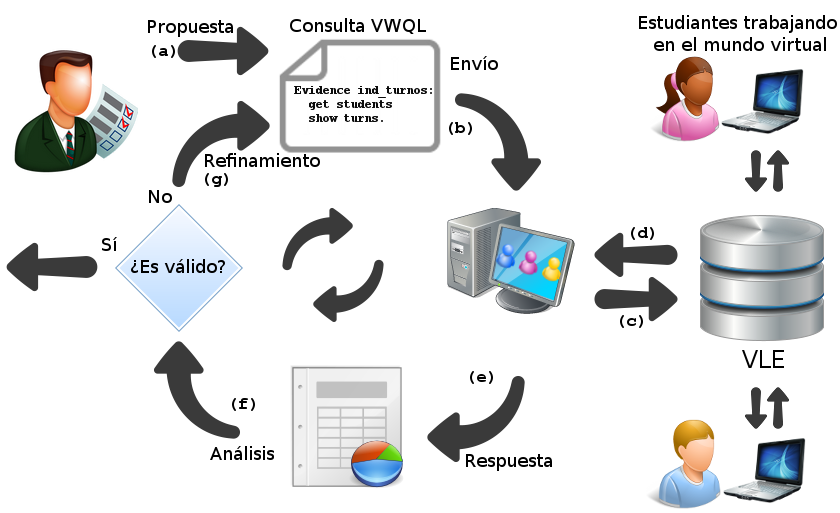
\includegraphics[scale=0.4]{EvsDiagram.png}
  \end{center}
  \caption{Ciclo de contraste de hipótesis con EvalSim}
  \label{fig:EvsDiagram}
\end{figure}

El profesor propone una evaluación (\emph{a}) que bajo su criterio le vaya a proporcionar indicadores válidos para evaluar alguna competencia genérica y la envía a EvalSim (\emph{b}). EvalSim procesa la petición y realiza la solicitud a la base de datos del mundo virtual (\emph{c}) . Una vez que recibe los datos (\emph{d}), los transforma y devuelve los resultados debidamente formateados al profesor (\emph{e}). El profesor los analiza, y si considera que son indicadores válidos para evaluar la competencia (\emph{f}) termina el ciclo. Sin embargo, si entiende que no les sirven o considera que debería refinarlo podría volver a diseñar una nueva evaluación (\emph{g}), reiniciándose de nuevo el ciclo.


\paragraph*{Ejemplo de uso}

En este ejemplo se parte de que el mundo virtual se está utilizando en una asignatura de idiomas. En un ejercicio práctico confeccionado por el profesor, los estudiantes han de participar en un juego de roles (\emph{role-play}) y son advertidos de que deben explayarse en sus respuestas a fin de utilizar los recursos lingüísticos aprendidos en clase.

Una vez que todos los estudiantes han participado el juego, el profesor decide utilizar como indicador el número de frases de una sola palabra utilizada por los estudiantes. De esta manera, todos aquellos estudiantes que hayan utilizado una sola palabra para responder a alguna pregunta tendrán una evaluación negativa en el desempeño de la competencia. Puede verse el código empleado en la consulta~\ref{code:vqwlej1}.

\begin{lstlisting}[caption=Respuestas de una sola palabra, label=code:vqwlej1,numbers=left, captionpos=b, morekeywords={Evidence,get, students, single, show, words, sentences, turns, time, points}]
Evidence respuestas_cortas:
    get students
    show single.
\end{lstlisting}

Como resultado a la consulta, el sistema devuelve el listado que puede verse en la tabla~\ref{tab:EvsListEj1}. A la vista de los mismos, el profesor considera que hay situaciones en las que una respuesta corta podría admitirse como válida, por lo que decide admitir como mucho dos respuestas cortas en la participación de cada estudiante. Ante este enfoque, el profesor considera que los estudiantes 3, 6 y 7 (\emph{studen3, student6 y student7}) tuvieron un desempeño bajo en la competencia al haber empleado cuatro, cuatro y tres respuestas cortas respectivamente.

\begin{table}
	\centering
	\caption{Información sobre las respuestas de una sola palabra dadas por los estudiantes en el role-play}
	\label{tab:EvsListEj1}
	\begin{tabular}{|l|l|c|}
		\hline
		id & username & singles \\
		\hline
		\hline
		1 & student1 & 0  \\
		\hline
		2 & student2 & 1  \\
		\hline
		3 & student3 & 4  \\
		\hline
		4 & student4 & 0  \\
		\hline
		5 & student5 & 2  \\
		\hline
		6 & student6 & 4  \\
		\hline
		7 & student7 & 3  \\
		\hline
		8 & student8 & 1  \\
		\hline
	\end{tabular}
\end{table}

Para enriquecer este indicador, el profesor decide diseñar un nuevo indicador. En este caso, calculando el número de palabras por turno que escriben los estudiantes. Para ello utiliza la consulta~\ref{code:vqwlej2}. Los resultados en este caso puede verse en la tabla~\ref{tab:EvsListEj2}.

\begin{lstlisting}[caption=Respuestas de una sola palabra, label=code:vqwlej2,numbers=left, captionpos=b, morekeywords={Evidence,get, students, single, show, words, sentences, turns, time, points}]
Evidence palabras_turno:
    get students
    show words, turns.
\end{lstlisting}

\begin{table}
	\centering
	\caption{Información sobre las palabras por turnos utilizadas por los estudiantes en el role-play}
	\label{tab:EvsListEj2}
	\begin{tabular}{|l|l|c|c|c|}
		\hline
		id & username & words & turns & words per turn \\
		\hline
		\hline
		1 & student1 & 117 & 9 & 13 \\
		\hline
		2 & student2 & 132 & 11 & 12  \\
		\hline
		3 & student3 & 63 & 9 & 7  \\
		\hline
		4 & student4 & 140 & 10 & 14  \\
		\hline
		5 & student5 & 99  & 11 & 9 \\
		\hline
		6 & student6 & 80 & 10 & 8  \\
		\hline
		7 & student7 & 72 & 9 & 8  \\
		\hline
		8 & student8 & 108 & 9 & 12   \\
		\hline
	\end{tabular}
\end{table}

A la vista de los resultados, el profesor confirma que los estudiantes 3, 6 y 7 (\emph{studen3, student6 y student7}) son los que utilizan menos palabras por turno. Son estos tres estudiantes, junto con el estudiante número 5 (\emph{student5}), los únicos que bajan de 10 palabras por turno. Lo que podría ser una justificación para el profesor a la hora de evaluar de manera negativa a este estudiante, ya que no sólo no llega a 10 mensajes sino que también es el único que en la consulta anterior está en el límite fijado de dos respuestas cortas.

Como en los casos anteriores, será decisión del profesor el uso que se dé a los indicadores.

\subsubsection{Indicadores}

El mundo virtual se ha desarrollado para asignaturas de idiomas, por lo que la competencia genérica para la que más se han utilizado los indicadores obtenidos ha sido para la \emph{habilidad para comunicarse en un segundo idioma}. Aunque sólo es una propuesta y podrían utilizarse también para otras competencias.

% Hipótesis: un estudiante tiene dificultades para hacerse entender si necesita dos o más frases por turno para comunicarse con su compañero.

\paragraph*{Segundo idioma}
\begin{itemize}
\item \emph{Ritmo}: número de frases escritas por minuto. Según la experiencia desarrollada podría ser un indicador positivo o negativo del desempeño de la competencia. Si el estudiante tiene que contar una historia o expresarse sin restricción, el hecho de que escriba muchas frases por minuto es un indicador positivo de su dominio del idioma. Sin embargo, si el estudiante tiene que enviar a su compañero un mensaje concreto y tiene dificultades  para hacerse entender, puede necesitar más de una frase por minuto para hacerse entender, siendo entonces un indicador negativo.
\item \emph{Frases por turno}: número de frases escritas por turno. Igual que en el caso anterior, puede tomarse como un indicador positivo o negativo dependiendo del caso. Si el estudiante tiene un buen dominio del idioma y no hay restricción impuesta, puede ser un indicador positivo que escriba muchas frases por turno. Mientras que si necesita muchas frases para transmitir un mensaje concreto, que tenga que escribir muchas frases por turno puede ser un indicador negativo del desempeño de la competencia.
\item \emph{Palabras solas}: número de frases de una sola palabra escritas por el estudiante. Un abuso del uso de frases de una sola palabra puede ser utilizado como un indicador del bajo nivel de conocimiento del segundo idioma.
\end{itemize}

\paragraph*{Capacidad de aprender y mantenerse al día con el aprendizaje}
Si un estudiante tiene dificultades para desenvolverse en el idioma, el hecho de que dedicase muchos minutos a jugar en el mundo virtual podría ser un indicador de que dicho estudiante está comprometido con su aprendizaje, y quiere mejorar. Sin embargo, si un estudiante tiene malos resultados, y además pasa pocos minutos practicando, sería un indicador negativo de esta competencia.
% La evaluación de las 3 herramientas se corresponde al capítulo siguiente.


%Metodología mixta

%Cómo voy a evaluar roles, momentos, actividad, ... lo que sea.

%Explicar el DSL

%DSL: herramienta de investigación en evaluaciones. Esta herramienta ayuda al investigador a formalizar la evaluación.
 
%Enfocar la metodología a que no es una metodología para evaluar, sino para diseñar evaluaciones. Diseñador de evaluaciones.

%Explicar qué pasos tiene que seguir un diseñador de evaluaciones para hacer sus evaluaciones.

%Dentro de los resultados obtenemos dos cosas:
%1. Diseño
%2. Lo que el diseñador nos indicó que no pudo hacer

%Para que esto sea posible falta la herramienta informática

%\section{Evolución herramientas}

%AMW --> EvalCourse --> EvalSim

%\section{Metodología de desarrollo}

%DSL? Ing. Dirigida x modelo?



%------------------------------------------------------------------------------------------------------------------------------------------------

